\documentclass{standalone}
\usepackage{tikz}
\usetikzlibrary{patterns, positioning}

\begin{document}
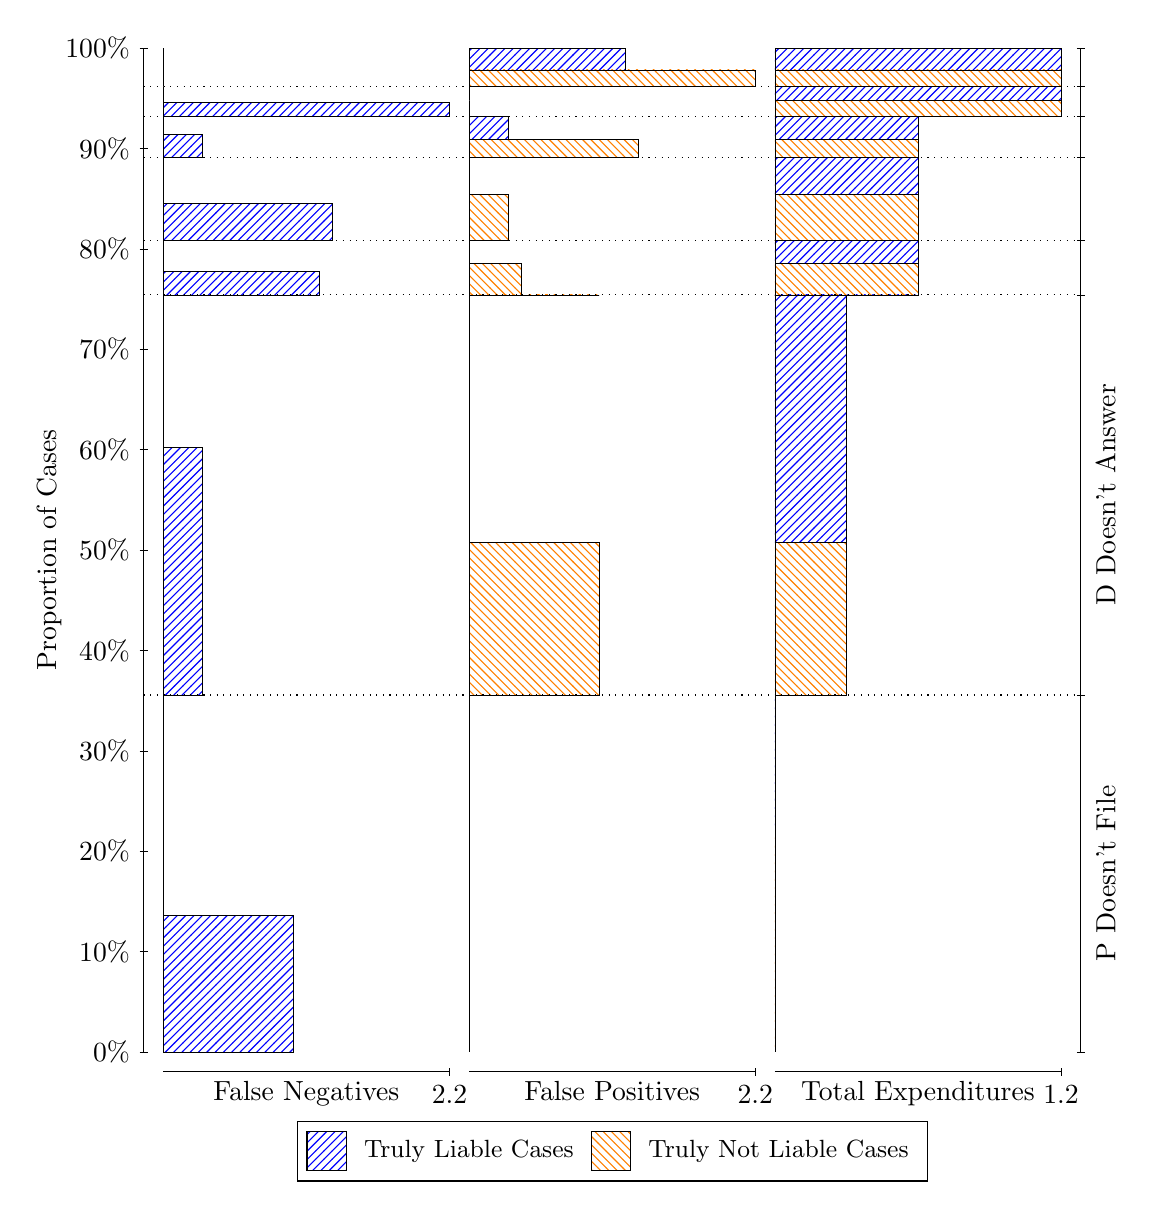
\begin{tikzpicture}
\draw[black, very thin] (1.5,1.75) -- (1.5,14.5);
\node[rotate=90, anchor=center] at (0.3, 8.125) {Proportion of Cases};
\draw[black, very thin] (1.45,1.75) -- (1.55,1.75);
\node[anchor=east] at (1.45, 1.75) {0\%};
\draw[black, very thin] (1.45,3.025) -- (1.55,3.025);
\node[anchor=east] at (1.45, 3.025) {10\%};
\draw[black, very thin] (1.45,4.3) -- (1.55,4.3);
\node[anchor=east] at (1.45, 4.3) {20\%};
\draw[black, very thin] (1.45,5.575) -- (1.55,5.575);
\node[anchor=east] at (1.45, 5.575) {30\%};
\draw[black, very thin] (1.45,6.85) -- (1.55,6.85);
\node[anchor=east] at (1.45, 6.85) {40\%};
\draw[black, very thin] (1.45,8.125) -- (1.55,8.125);
\node[anchor=east] at (1.45, 8.125) {50\%};
\draw[black, very thin] (1.45,9.4) -- (1.55,9.4);
\node[anchor=east] at (1.45, 9.4) {60\%};
\draw[black, very thin] (1.45,10.675) -- (1.55,10.675);
\node[anchor=east] at (1.45, 10.675) {70\%};
\draw[black, very thin] (1.45,11.95) -- (1.55,11.95);
\node[anchor=east] at (1.45, 11.95) {80\%};
\draw[black, very thin] (1.45,13.225) -- (1.55,13.225);
\node[anchor=east] at (1.45, 13.225) {90\%};
\draw[black, very thin] (1.45,14.5) -- (1.55,14.5);
\node[anchor=east] at (1.45, 14.5) {100\%};

\draw[black, very thin] (13.4,1.75) -- (13.4,14.5);
\draw[black, very thin] (13.35,1.75) -- (13.45,1.75);
\node[anchor=west] at (13.35, 1.75) {};
\draw[black, very thin] (13.35,6.284) -- (13.45,6.284);
\node[anchor=west] at (13.35, 6.284) {};
\draw[black, very thin] (13.35,11.366) -- (13.45,11.366);
\node[anchor=west] at (13.35, 11.366) {};
\draw[black, very thin] (13.35,12.059) -- (13.45,12.059);
\node[anchor=west] at (13.35, 12.059) {};
\draw[black, very thin] (13.35,13.113) -- (13.45,13.113);
\node[anchor=west] at (13.35, 13.113) {};
\draw[black, very thin] (13.35,13.633) -- (13.45,13.633);
\node[anchor=west] at (13.35, 13.633) {};
\draw[black, very thin] (13.35,14.01) -- (13.45,14.01);
\node[anchor=west] at (13.35, 14.01) {};
\draw[black, very thin] (13.35,14.5) -- (13.45,14.5);
\node[anchor=west] at (13.35, 14.5) {};

\draw[black, very thin, pattern color=blue, pattern=north east lines] (1.75,1.75) rectangle (3.4015,3.4804);
\draw[black, very thin, pattern color=orange, pattern=north west lines] (1.75,3.4804) rectangle (1.75,6.284);
\draw[black, very thin, pattern color=blue, pattern=north east lines] (1.75,6.284) rectangle (2.2455,9.424);
\draw[black, very thin, pattern color=orange, pattern=north west lines] (1.75,9.424) rectangle (1.75,11.366);
\draw[black, very thin, pattern color=blue, pattern=north east lines] (1.75,11.366) rectangle (3.7318,11.66);
\draw[black, very thin, pattern color=blue, pattern=north east lines] (1.75,11.66) rectangle (3.4015,11.66);
\draw[black, very thin, pattern color=blue, pattern=north east lines] (1.75,11.66) rectangle (3.2364,11.66);
\draw[black, very thin, pattern color=blue, pattern=north east lines] (1.75,11.66) rectangle (3.2364,11.66);
\draw[black, very thin, pattern color=blue, pattern=north east lines] (1.75,11.66) rectangle (3.0712,11.66);
\draw[black, very thin, pattern color=blue, pattern=north east lines] (1.75,11.66) rectangle (2.9061,11.66);
\draw[black, very thin, pattern color=blue, pattern=north east lines] (1.75,11.66) rectangle (2.7409,11.66);
\draw[black, very thin, pattern color=orange, pattern=north west lines] (1.75,11.66) rectangle (1.75,12.059);
\draw[black, very thin, pattern color=blue, pattern=north east lines] (1.75,12.059) rectangle (3.897,12.526);
\draw[black, very thin, pattern color=orange, pattern=north west lines] (1.75,12.526) rectangle (1.75,13.113);
\draw[black, very thin, pattern color=blue, pattern=north east lines] (1.75,13.113) rectangle (2.2455,13.403);
\draw[black, very thin, pattern color=orange, pattern=north west lines] (1.75,13.403) rectangle (1.75,13.633);
\draw[black, very thin, pattern color=blue, pattern=north east lines] (1.75,13.633) rectangle (5.3833,13.808);
\draw[black, very thin, pattern color=orange, pattern=north west lines] (1.75,13.808) rectangle (1.75,14.01);
\draw[black, very thin, pattern color=orange, pattern=north west lines] (1.75,14.01) rectangle (1.75,14.222);
\draw[black, very thin, pattern color=blue, pattern=north east lines] (1.75,14.222) rectangle (1.75,14.5);
\draw[black, very thin, pattern color=orange, pattern=north west lines] (5.6333,1.75) rectangle (5.6333,4.5536);
\draw[black, very thin, pattern color=blue, pattern=north east lines] (5.6333,4.5536) rectangle (5.6333,6.284);
\draw[black, very thin, pattern color=orange, pattern=north west lines] (5.6333,6.284) rectangle (7.2848,8.2261);
\draw[black, very thin, pattern color=blue, pattern=north east lines] (5.6333,8.2261) rectangle (5.6333,11.366);
\draw[black, very thin, pattern color=orange, pattern=north west lines] (5.6333,11.366) rectangle (7.2848,11.366);
\draw[black, very thin, pattern color=orange, pattern=north west lines] (5.6333,11.366) rectangle (7.1197,11.366);
\draw[black, very thin, pattern color=orange, pattern=north west lines] (5.6333,11.366) rectangle (6.9545,11.366);
\draw[black, very thin, pattern color=orange, pattern=north west lines] (5.6333,11.366) rectangle (6.7894,11.366);
\draw[black, very thin, pattern color=orange, pattern=north west lines] (5.6333,11.366) rectangle (6.6242,11.366);
\draw[black, very thin, pattern color=orange, pattern=north west lines] (5.6333,11.366) rectangle (6.2939,11.765);
\draw[black, very thin, pattern color=blue, pattern=north east lines] (5.6333,11.765) rectangle (5.6333,12.059);
\draw[black, very thin, pattern color=orange, pattern=north west lines] (5.6333,12.059) rectangle (6.1288,12.646);
\draw[black, very thin, pattern color=blue, pattern=north east lines] (5.6333,12.646) rectangle (5.6333,13.113);
\draw[black, very thin, pattern color=orange, pattern=north west lines] (5.6333,13.113) rectangle (7.7803,13.343);
\draw[black, very thin, pattern color=blue, pattern=north east lines] (5.6333,13.343) rectangle (6.1288,13.633);
\draw[black, very thin, pattern color=orange, pattern=north west lines] (5.6333,13.633) rectangle (5.6333,13.835);
\draw[black, very thin, pattern color=blue, pattern=north east lines] (5.6333,13.835) rectangle (5.6333,14.01);
\draw[black, very thin, pattern color=orange, pattern=north west lines] (5.6333,14.01) rectangle (9.2667,14.222);
\draw[black, very thin, pattern color=blue, pattern=north east lines] (5.6333,14.222) rectangle (7.6152,14.5);
\draw[black, very thin, pattern color=orange, pattern=north west lines] (9.5167,1.75) rectangle (9.5167,4.5536);
\draw[black, very thin, pattern color=blue, pattern=north east lines] (9.5167,4.5536) rectangle (9.5167,6.284);
\draw[black, very thin, pattern color=orange, pattern=north west lines] (9.5167,6.284) rectangle (10.425,8.2261);
\draw[black, very thin, pattern color=blue, pattern=north east lines] (9.5167,8.2261) rectangle (10.425,11.366);
\draw[black, very thin, pattern color=orange, pattern=north west lines] (9.5167,11.366) rectangle (11.333,11.366);
\draw[black, very thin, pattern color=blue, pattern=north east lines] (9.5167,11.366) rectangle (11.333,11.366);
\draw[black, very thin, pattern color=orange, pattern=north west lines] (9.5167,11.366) rectangle (11.333,11.765);
\draw[black, very thin, pattern color=blue, pattern=north east lines] (9.5167,11.765) rectangle (11.333,12.059);
\draw[black, very thin, pattern color=orange, pattern=north west lines] (9.5167,12.059) rectangle (11.333,12.059);
\draw[black, very thin, pattern color=blue, pattern=north east lines] (9.5167,12.059) rectangle (11.333,12.059);
\draw[black, very thin, pattern color=orange, pattern=north west lines] (9.5167,12.059) rectangle (11.333,12.646);
\draw[black, very thin, pattern color=blue, pattern=north east lines] (9.5167,12.646) rectangle (11.333,13.113);
\draw[black, very thin, pattern color=orange, pattern=north west lines] (9.5167,13.113) rectangle (11.333,13.343);
\draw[black, very thin, pattern color=blue, pattern=north east lines] (9.5167,13.343) rectangle (11.333,13.633);
\draw[black, very thin, pattern color=orange, pattern=north west lines] (9.5167,13.633) rectangle (13.15,13.835);
\draw[black, very thin, pattern color=blue, pattern=north east lines] (9.5167,13.835) rectangle (13.15,14.01);
\draw[black, very thin, pattern color=orange, pattern=north west lines] (9.5167,14.01) rectangle (13.15,14.222);
\draw[black, very thin, pattern color=blue, pattern=north east lines] (9.5167,14.222) rectangle (13.15,14.5);
\draw[black, dotted] (1.5,6.284) -- (13.4,6.284);
\draw[black, dotted] (1.5,11.366) -- (13.4,11.366);
\draw[black, dotted] (1.5,12.059) -- (13.4,12.059);
\draw[black, dotted] (1.5,13.113) -- (13.4,13.113);
\draw[black, dotted] (1.5,13.633) -- (13.4,13.633);
\draw[black, dotted] (1.5,14.01) -- (13.4,14.01);
\draw[black, very thin] (1.75,1.5) -- (5.3833,1.5);
\node[anchor=north] at (3.5667, 1.5) {False Negatives};
\draw[black, very thin] (5.3833,1.45) -- (5.3833,1.55);
\node[anchor=north] at (5.3833, 1.45) {2.2};

\draw[black, very thin] (5.6333,1.5) -- (9.2667,1.5);
\node[anchor=north] at (7.45, 1.5) {False Positives};
\draw[black, very thin] (9.2667,1.45) -- (9.2667,1.55);
\node[anchor=north] at (9.2667, 1.45) {2.2};

\draw[black, very thin] (9.5167,1.5) -- (13.15,1.5);
\node[anchor=north] at (11.333, 1.5) {Total Expenditures};
\draw[black, very thin] (13.15,1.45) -- (13.15,1.55);
\node[anchor=north] at (13.15, 1.45) {1.2};

\node[black, centered, rotate=90] at (13.72, 4.017) {P Doesn't File};
\node[black, centered, rotate=90] at (13.72, 8.8251) {D Doesn't Answer};






\draw (7.449999999999999,1.5) node[draw=none] (baseCoordinate) {};
\begin{scope}[align=center]
        \matrix[scale=0.5, draw=black, below=0.5cm of baseCoordinate, nodes={draw}, column sep=0.1cm]{
            \node[rectangle, draw, minimum width=0.5cm, minimum height=0.5cm, pattern=north east lines, pattern color=blue] {}; &
            \node[draw=none, font=\small] (B) {Truly Liable Cases}; &
            \node[rectangle, draw, minimum width=0.5cm, minimum height=0.5cm, pattern=north west lines, pattern color=orange] {}; &
            \node[draw=none, font=\small] (B) {Truly Not Liable Cases}; \\
            };
\end{scope}

\end{tikzpicture}
\end{document}